% !Mode:: "TeX:UTF-8"

\chapter[相关理论和技术介绍]{背景知识和相关技术介绍}[xxx]
% 10-11页
\section{引言}
本章将会对利用变分自编码器进行交通数据缺失值填充所需要的前置知识进行介绍。本章首先介绍城市交通网络中出现的一些重要的名词定义,然后介绍了神经网络中常用的卷积运算,接着介绍了标准化流技术,最后本章着重描述了用于重建数据的原始变分自编码器模型。
\section{城市交通网络相关理论}
\subsection{交通栅格数据}
交通流量是城市交通网络的重要组成部分,它提供了特定路段或区域中的空间拥堵信息,这在城市网络分析中十分重要,因为交通流量的大小会影响交通工具的行驶时间,从而影响交通管制单位的行为决策或城市居民的出行计划。

根据不同的粒度和语义信息可以对一个区域做出多种定义,本文中主要采用以下的方式来定义城市交通区域。
\begin{definition}[\cite{zhang2017deep}(区域)] 将一个城市的经纬度转化成平面坐标,并按照规定间距等距离将整个城市地图划分为长为$H$,宽为$W$的网格图$\mathcal{G}$,图中的每个格子$(h, w)$代表一个区域,如图\ref{gridmap}所示。

\end{definition}
\begin{figure}[h]
\centering
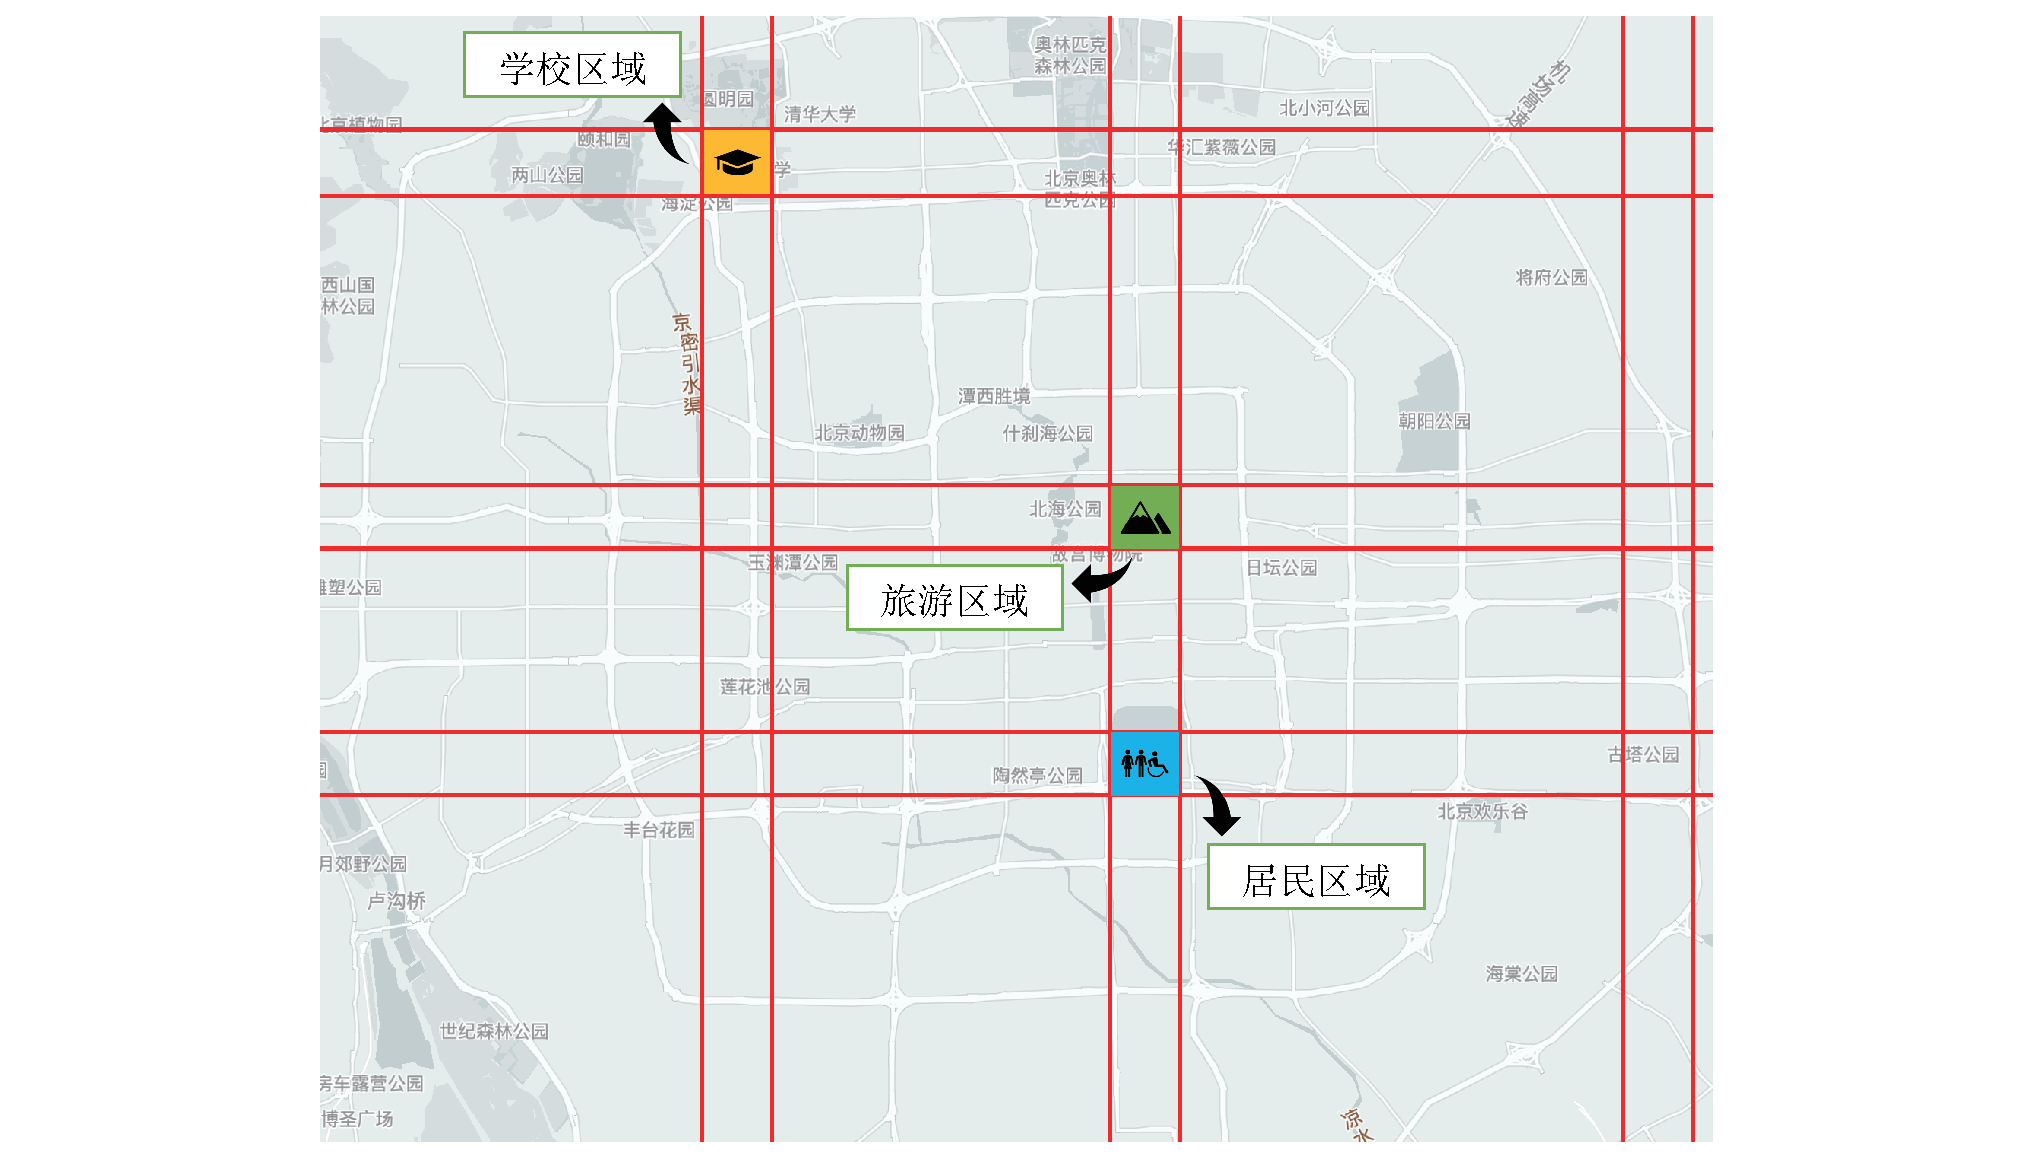
\includegraphics[width = 0.9\textwidth]{gridmap}
\vspace{0.5em}
\caption{城市区域网格图 \label{gridmap}}
\end{figure}

\begin{definition}[\cite{zhang2017deep}(区域出入流量)] \label{def_flow}
给定第$t$个时间区间内的人群轨迹集合$\mathbb{P}_{t}$,在图$\mathcal{G}$的区域$(h, w)$内,区域交通出入流量可以分别用下式定义。
\begin{equation}
	x^{in, t, h, w} = \sum_{Tr_{t} \in \mathbb{P}_{t}}\left|\left\{k>1 \mid l_{k-1} \notin(h, w) \wedge l_{k} \in(h, w)\right\}\right|
\end{equation}
\begin{equation}
	x^{out, t, h, w} = \sum_{Tr_{t} \in \mathbb{P}_{t}}\left|\left\{k \geq 1 \mid l_{k-1} \in(h, w) \wedge l_{k} \notin(h, w)\right\}\right|,
\end{equation}
其中$Tr_{t}: l_{1} \rightarrow l_{2} \rightarrow \cdots \rightarrow l_{|Tr_t|}$表示集合$\mathbb{P}_t$中的一条轨迹,且$l_k$表示地理坐标;$l_k \in(h, w)$表示坐标$l_k$位于区域$(h, w)$内,反之亦然;$| \cdot |$表示集合的基数。
\end{definition}

\begin{figure}[htbp]
\centering
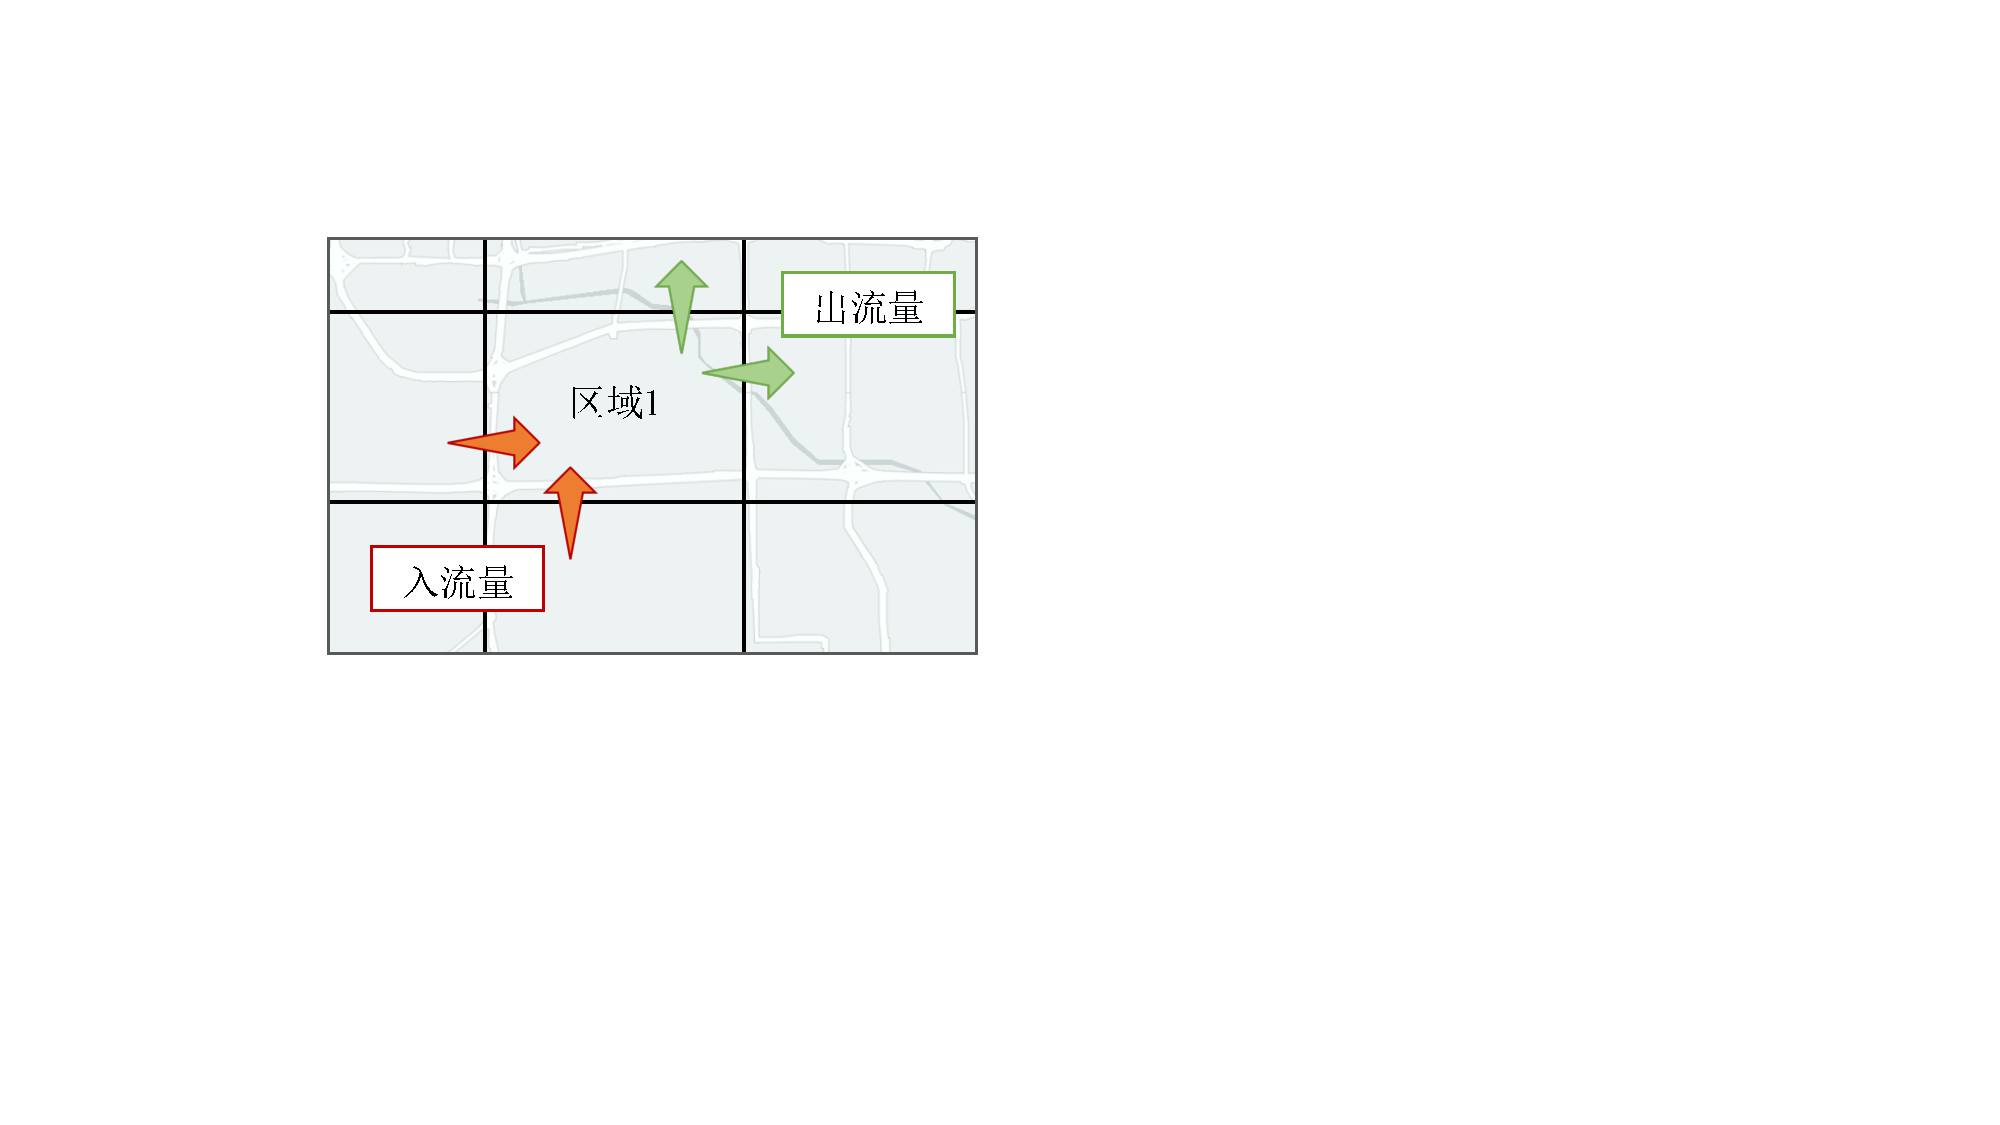
\includegraphics[width = 0.4\textwidth]{region}
\vspace{0.5em}
\caption{区域出入流量 \label{region}}
\end{figure}
也就是说,区域入流量是指在给定的时间区间内从其他地点进入此区域的人流量总数,区域出流量是指在给定的时间区间内从该区域离开的人流量总数,如图\ref{region}所示。两个指标记录了不同区域间人群的转移情况,因此,挖掘其中的信息对于交通管制和交通风险评估意义重大。区域出入流量可由交通工具数量、路上行人数等统计得到,常用的测量手段有使用手机信号来定位行人的轨迹、使用GPS来定位出租车的位置,图\ref{measure}给出了形象的描述。

\begin{figure}[htbp]
\centering
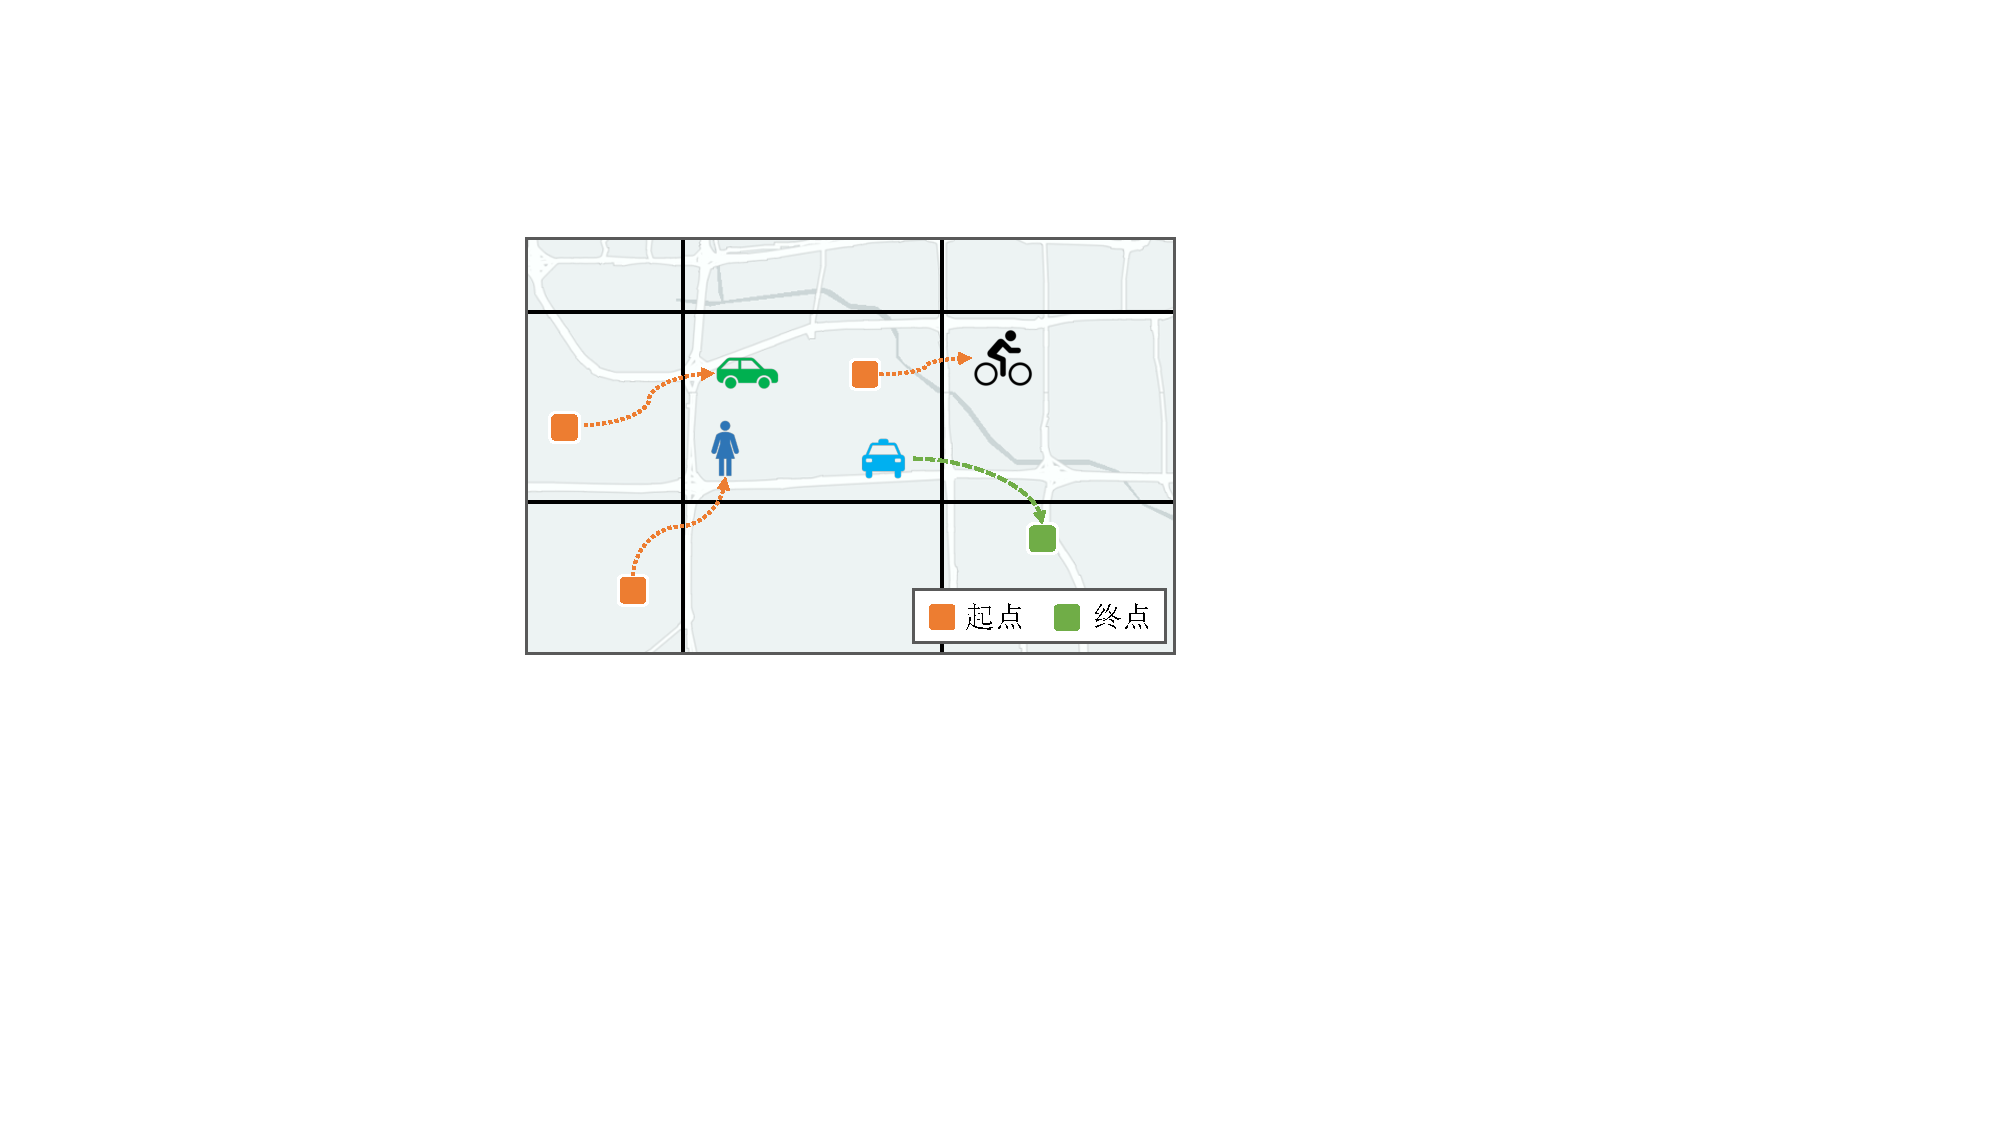
\includegraphics[width = 0.5\textwidth]{measure}
\vspace{0.5em}
\caption{交通流量测量 \label{measure}}
\end{figure}

%\begin{figure}[htbp]
%\centering
%\begin{minipage}[t]{0.42\textwidth}
%\centering
%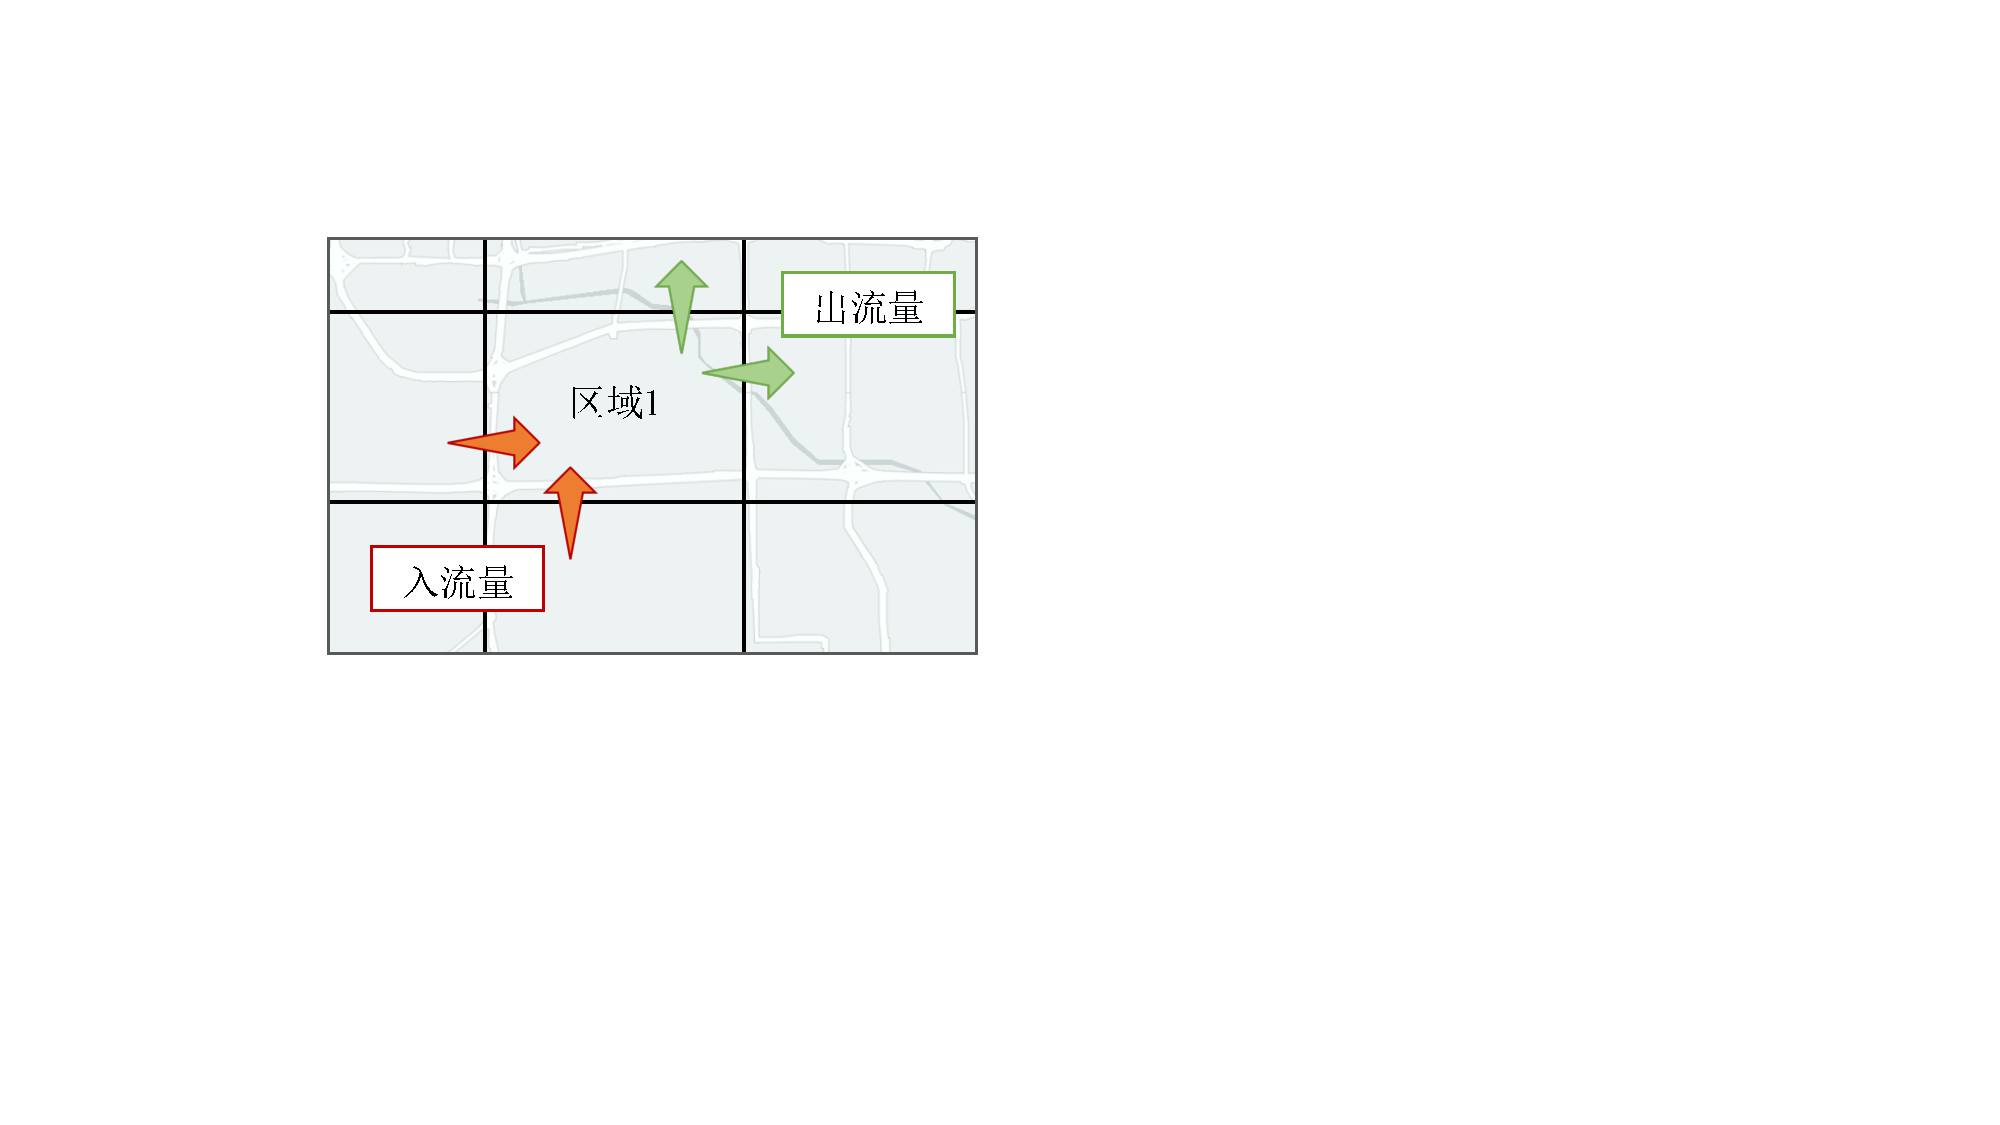
\includegraphics[width=\textwidth]{region}
%%\vspace{0.1em}
%\caption{区域出入流量 \label{region}}
%\end{minipage}
%\centering
%\begin{minipage}[t]{0.42\textwidth}
%\centering
%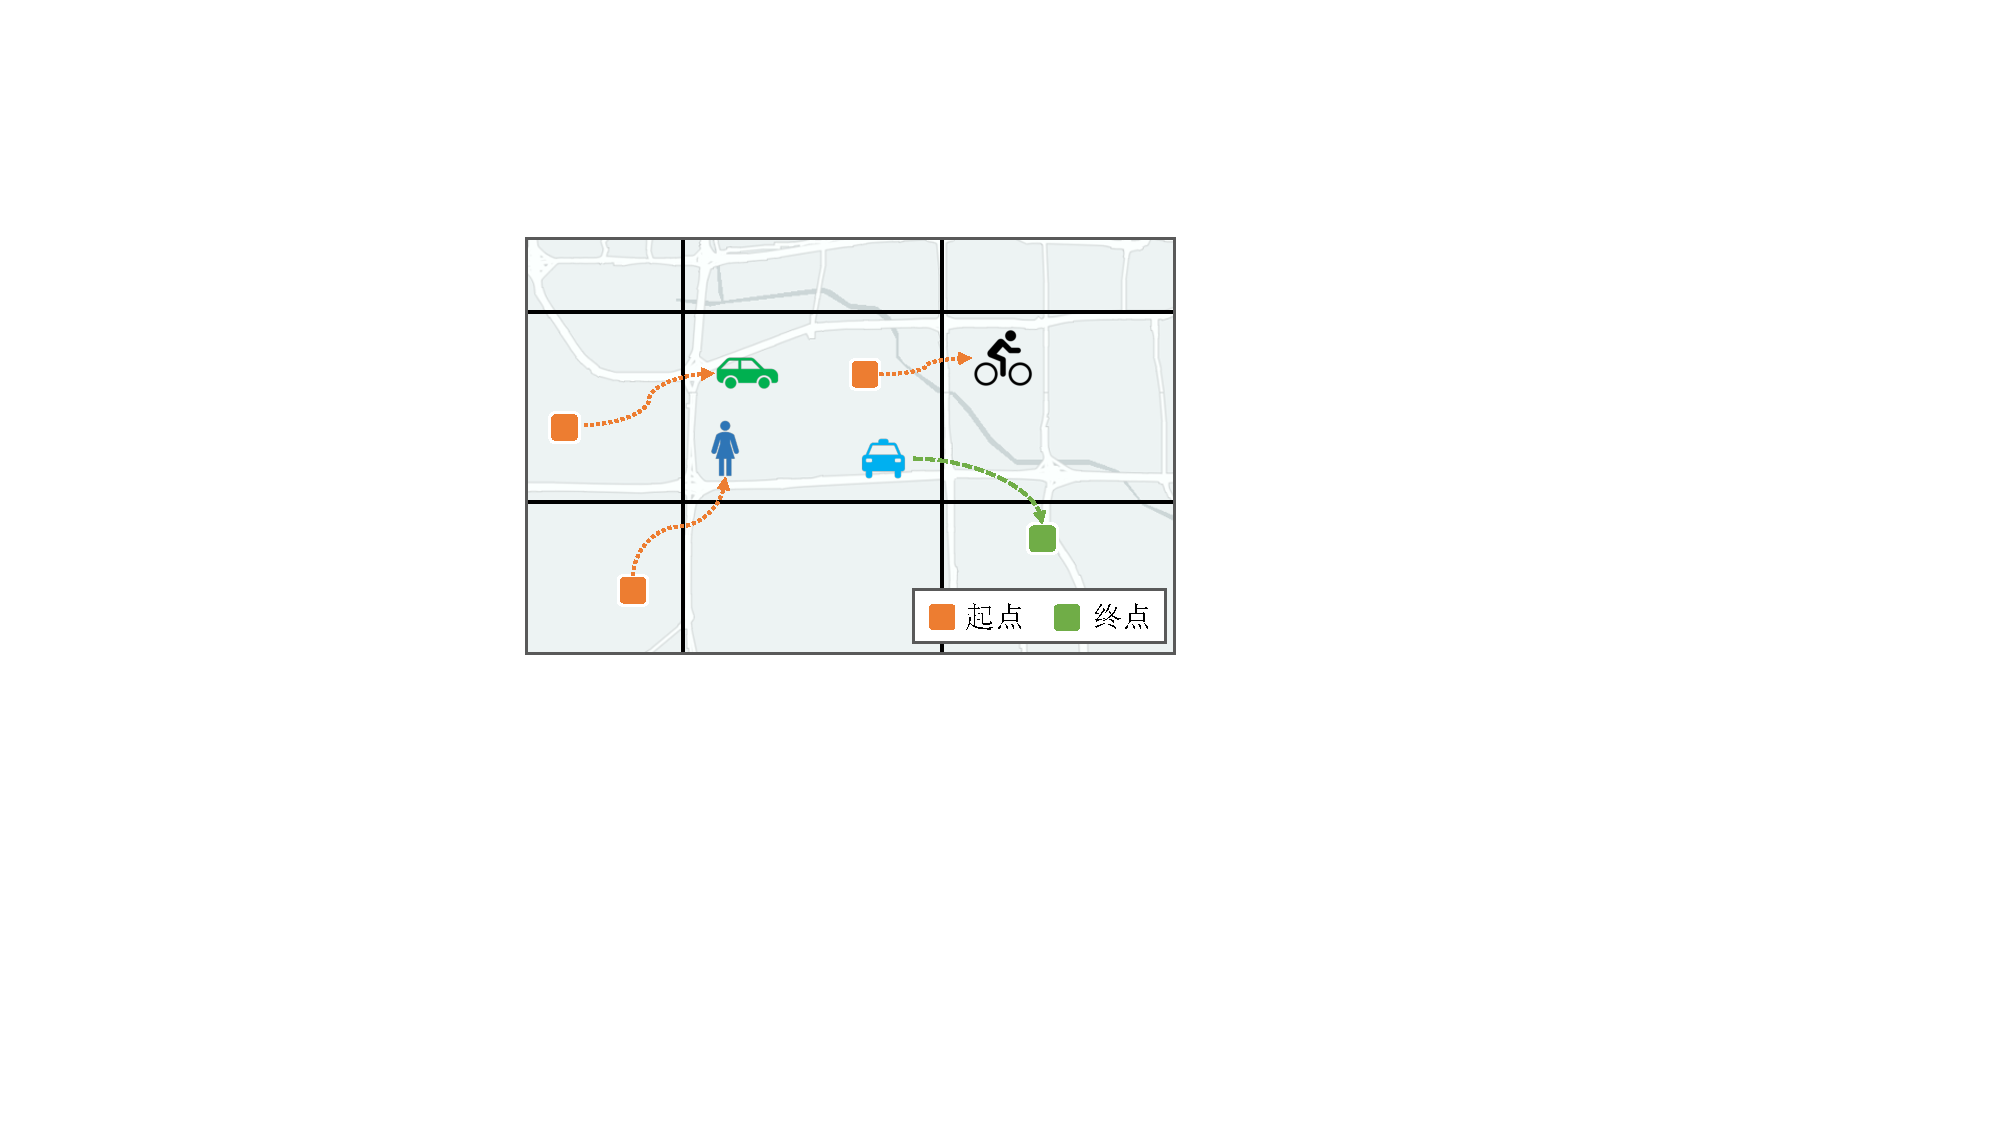
\includegraphics[width=\textwidth]{measure}
%%\vspace{0.1em}
%\caption{交通流量测量 \label{measure}}
%\end{minipage}
%\end{figure}

Atluri\cite{atluri2018spatio}等人将时空数据分为四大类,分别包括事件数据、轨迹数据、点参考数据和栅格数据。本文将人群轨迹数据转换成栅格数据,即在第$t$个时间区间内,图$\mathcal{G}$内所有的交通出入流量可以被表示成一个张量$x_t\in\mathbb{R}^{2 \times H \times W}$,其中$x_t[0,h,w]=x^{in,t,h,w}$,$x_t[1,h,w]=x^{out,t,h,w}$。

\subsection{数据缺失机制}
文献\inlinecite{little2019statistical}指出,缺失值填充过程旨在学习未被观测到的缺失数据的概率分布,一般可将缺失值的缺失模式分为以下三种情况:

(1)完全随机缺失(Missing Completely At Random,MCAR)。该缺失模式是指缺失值的产生是完全随机的,即数据的缺失的概率分布独立于任何观测变量和其它缺失变量。本文通过采用百分位阈值的方式,随机采样固定百分比的位置作为缺失值来模拟该机制。

(2)随机缺失(Missing At Random,MAR)。该缺失模式缺失值的产生不是完全随机的,即缺失值依赖于其它观测变量,但不依赖于缺失变量。

(3)非随机缺失(Missing Not At Random,MNAR)。该缺失模式缺失值的产生依赖于观测变量和缺失变量自身。它一般由传感器的长期故障所导致,故无法通过算法来很好地还原原始数据,本文不考虑此种缺失模式。


%\section{神经网络激活函数}
%神经网络中的全连接层相当于对数据进行仿射变换,那么叠加多个全连接层的效果等价于将其压缩成一个全连接层,这样增加网络层数并不能提升网络的拟合能力,因此有必要在层与层之间添加非线性的激活函数来强化神经网络的学习能力。以下公式介绍了本文中所用到的激活函数。
%\begin{equation}
%	Sigmoid(x)=\frac{1}{1+e^{-x}}
%\end{equation}
%\begin{equation}
%	Tanh(x)=\frac{e^x-e^{-x}}{e^x+e^{-x}}
%\end{equation}
%\begin{equation}
%	ReLU(x)=max(0, x)
%\end{equation}
%\begin{equation}
%LeakyReLU(x)=
%\begin{cases}
%x, & x>0\\
%-\alpha x, & x \le 0, \alpha \textgreater 0.
%\end{cases}
%\end{equation}
%
%在本文的研究工作中,主要将$Sigmoid$函数和$Tanh$函数用于输入和输出数据值域的缩放,而$ReLU$函数\cite{krizhevsky2012imagenet}和$LeakyReLU$函数\cite{maas2013rectifier}则用于神经网络内部,主要原因是后两者解决了前者梯度消失的问题,且能加速模型的计算速度。

\section{卷积运算}
卷积神经网络一直是深度学习蓬勃发展的核心,但它与全连接网络不同,它的输出不仅取决于输入的大小,还取决于网络层内部多个参数的设定,因此,有必要对其进行介绍。下面将对普通2D卷积、转置卷积、3D卷积进行阐述。
\subsection{普通卷积和转置卷积}
从数学定义的角度来看,普通卷积是为了诸如信号处理,求两个随机变量和的分布等而定义的运算。并且,数学定义中的卷积核的值是已经被确定了,因此需要将卷积核(权重矩阵)翻转后,再同原来的矩阵数据作对乘操作,同时按照一定的操作顺序(即从上到下,从左到右的顺序),在原始的矩阵数据上进行重复滑动计算。在深度学习中,普通卷积的卷积核的值可以通过神经网络的反向传播进行学习,因而在深度学习中的卷积核并没有翻转这一操作。一个卷积核对应一个矩阵变换操作,多个卷积核对应多个函数映射操作,可以拓展到多个随机分布,这样可以从输入的矩阵数据中提取到更多的随即特征。同时,卷积核权重的更新过程可以看成是一个复杂函数拟合的过程。

\vspace{1em}
\begin{figure}[htbp] 
\centering
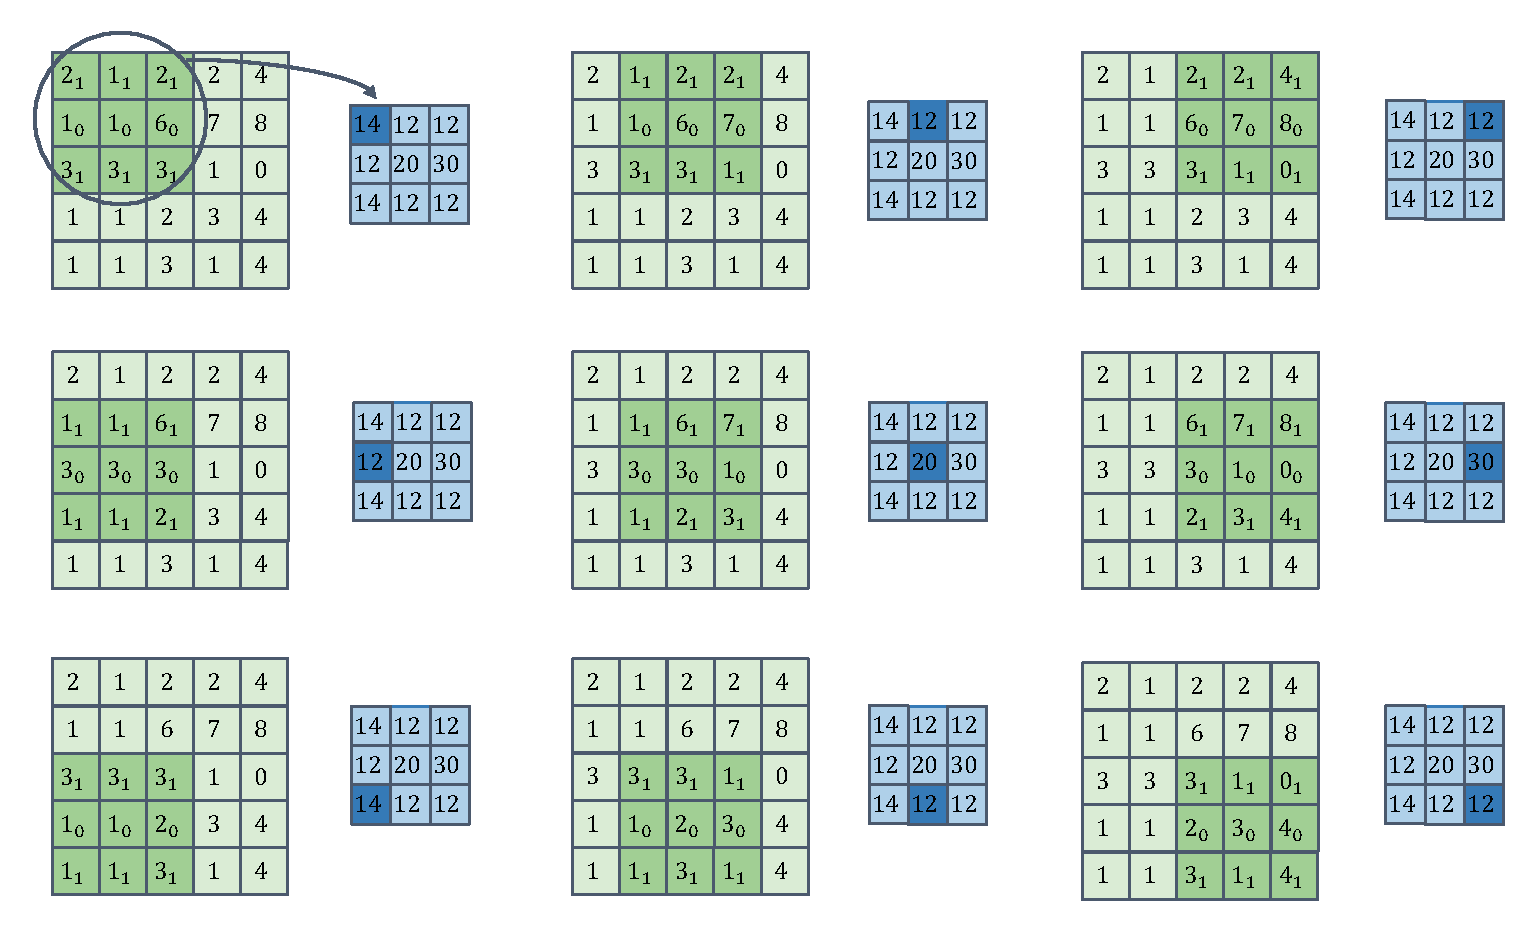
\includegraphics[width = \textwidth]{conv}
\vspace{-0.5em}
\caption{2D卷积运算\label{conv2d}} 
\end{figure}

其运算形式如下所示:
\begin{equation}
	O(i, j) = \sum_{m} \sum_{n} F(m, n) I(i+m, j+n).
\end{equation}

转置卷积(Transposed Convolution)与一般也叫做反卷积,其具体的操作过程如图\ref{tranconv}所示。。它通常用于将输入的特征图进行放大还原成原始大小。因而经常与卷积操作进行组合。卷积加上转置卷积的基础模型,也叫做自编码器。虽说转置卷积的操作结果是将卷积操作处理得到的特征图还原为原始数据大小,但是这并不意味着转置卷积就是卷积的反向操作。因为即使在普通卷积上使用同一个卷积核进行操作,也不可能保证得到的结果就和原始数据的一模一样。转置卷积的操作一般是先按照一定的比例通过填充补零的操作来扩大输入图像的尺寸,接着再按照一定的顺序(即从上到下,从左到右的顺序),移动卷积核,在进行普通卷积得到相应的结果。过程如图\ref{tranconv}所示。

\begin{figure}[htbp]
\centering
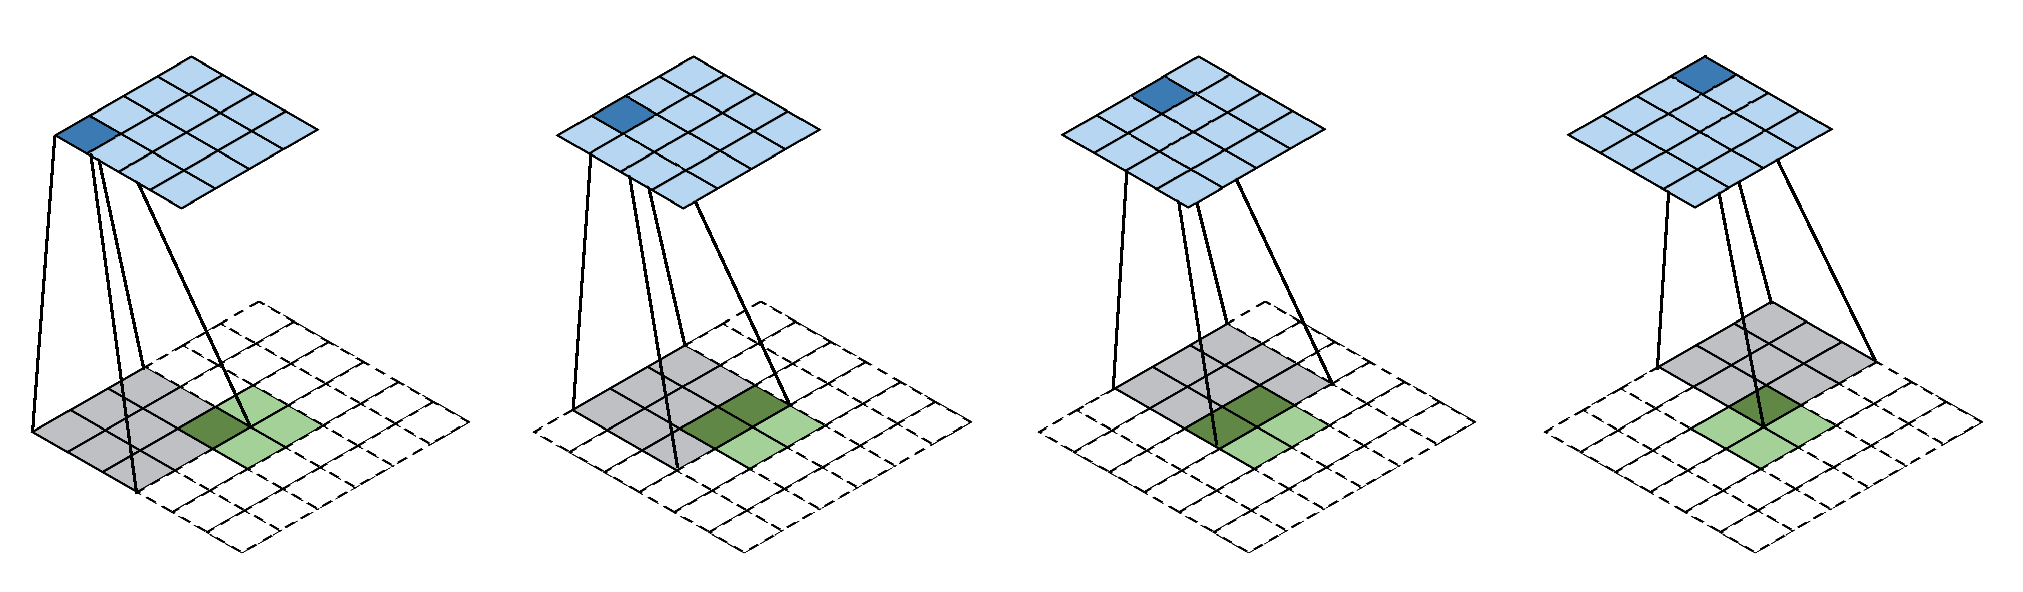
\includegraphics[width = \textwidth]{transpose_conv}
\vspace{0.25em}
\caption{转置卷积过程 \label{tranconv}}
\end{figure}

对一个输入图线进行转置卷积操作后得到的特征图$O$的尺寸$H_{out}$可由如下式子计算得出:
\begin{equation}
	H_{out}=(H_{in}-1)s - 2p+k,
\end{equation}
基于转置卷积能恢复形状的特性,它被广泛应用于图像的上采样操作,尤其在自编码器结构中的解码器和生成对抗网络中的生成器中使用较为频繁。

\subsection{3D卷积}
从前面的介绍中可以得知,2D卷积(即普通卷积)主要用于处理二维数据,比如静态图片,时序数据等。当使用2D卷积处理类似视频这些连续的图像数据,或者其它时空数据时,就需要把数据压缩成二维数据。最常使用的方式主要是把RGB通道维度同时间维度压缩成一个单维度。但是这样却会使得卷积无法准确地区分通道特征和时间特征,导致无法获取到准确的特征。3D卷积于2010年被Shuiwang Ji团队\cite{ji20123d}所提出,主要是应用在处理时空数据的特征提取问题上。

如图\ref{3Dconv}所示,3D卷积的卷积核比2D卷积多了一个时间维度,因此能保留输入图像的时间信息。

对一个输入视频进行3D卷积操作,一般需要指定以下参数:

(1)输入视频$I$的尺寸$W_{in}$

(2)卷积核$F$的尺寸$k$

(3)填充(padding)大小$p$

(4)步长(stride)大小$s$

那么经过3D卷积运算后得到的特征图$O$的尺寸$W_{out}$可由如下式子计算得出:
\begin{equation}
	W_{out}=\bigg{\lfloor} \frac{W_{in}+2p-k}{s} \bigg{\rfloor} + 1,
\end{equation}

另外$O$中每一个元素$O(t,i,j)$可由以下卷积操作计算得出:
\begin{equation}
	O(t, i, j) = \sum_{l} \sum_{m} \sum_{n} F(l, m, n) I(t+l, i+m, j+n).
\end{equation}

自从3D卷积被提出来后,它就被广泛应用于行为识别\cite{tran2018closer},视频修复\cite{wang2019video}等领域。同样的,交通数据作为一种常见的时空数据,也包含了时间维度,以及空间维度。因而可以将3D卷积应用于叫用数据挖掘任务\cite{yu20193d, guo2019deep}。
\begin{figure}[htbp] 
\centering
\includegraphics[width = 0.6\textwidth]{3Dconv}
\caption{3D卷积 \label{3Dconv}}
\end{figure}

\section{ConvGRU}
由于RNN系列模型(包括GRU模型以及LSTM模型)在处理时序数据时的优越表现,因而它被广泛应用到与时序相关的问题中,比如股价预测问题等。普通的GRU模型是在LSTM模型的基础上将相关门电路的功能进行整合简化,只保留了重置门电路和更新门电路。极大程度上降低了模型的训练难度。GRU模型的更新公式如下所示:

虽然RNN系列模型在处理时序数据时表现出优越的性能。但是由于其自身模型的设计,即在神经元的连接部分使用全连接层处理数据。限制了它处理时空数据的能力。为了使得RNN系列模型能够进一步处理时空数据这种三维数据。Shixingjian博士团队提出了新的RNN系列模型ConvLSTM以及ConvGRU模型。ConvGRU模型的改进之处主要是将模型中的全连接操作更换为卷积操作,从而使得模型具备处理时空数据的能力。ConvGRU模型的更新公式如下:

自从新的RNN系列模型ConvLSTM以及ConvGRU模型被提出来之后,它就被广泛应用到天气预测问题,以及视频预测等一系列时空数据的问题中。交通数据作为一种寻常的时空数据,ConvGRU模型也可以应用到交通数据的缺失值填充问题中。

\section{标准化流技术}
标准化流(Normalizing Flows)的核心思想是将一个相对简单,也就是易于采样的概率分布通过一系列可逆的参数化转换映射成一个更加灵活的概率分布,如图\ref{normal_flow}所示。下面介绍如何计算一个随机变量的概率密度函数,该随机变量由另外的随机变量变换而来。

\begin{figure}[htbp]
\centering
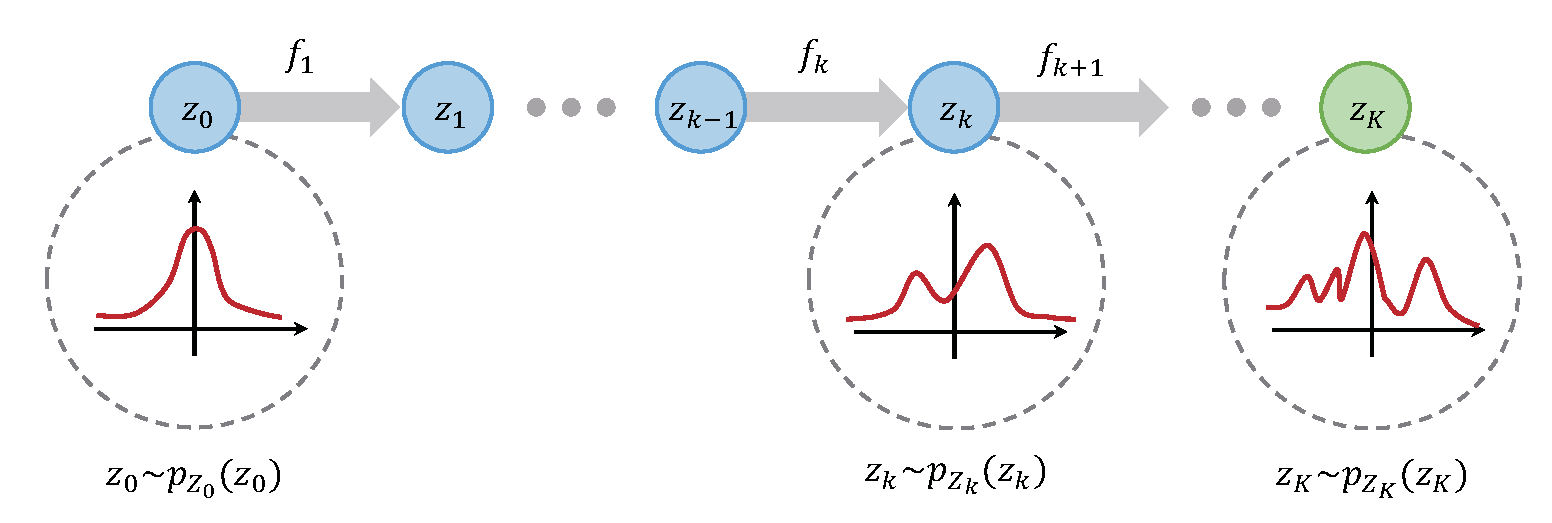
\includegraphics[width = 0.9\textwidth]{flow}
\vspace{1em}
\caption{标准化流 \label{normal_flow}}
\end{figure}

假设随机变量$Z \in \mathbb{R}^n$的概率密度函数已知且易于计算(Tractable),记为$p_Z: \mathbb{R}^n \rightarrow \mathbb{R}$,另一个待求的随机变量$X \in \mathbb{R}^n$密度函数为$p_X: \mathbb{R}^n \rightarrow \mathbb{R}$,二者之间存在可逆的映射关系$f:\mathbb{R}^n \rightarrow \mathbb{R}^n$,即满足$X=f(Z)$且$Z=f^{-1}(X)$,则有
\begin{equation}
\begin{split}
	p_X(x) & = p_Z(f^{-1}(x))\bigg | det\bigg (\frac{\partial f^{-1}(x)}{\partial x}\bigg )\bigg | \\
	& = p_Z(z)\bigg | det\bigg (\frac{\partial f(z)}{\partial z}\bigg )\bigg |^{-1}, \\
\end{split}
\end{equation}
其中,$\frac{\partial f^{-1}(x)}{\partial x}$和$\frac{\partial f(z)}{\partial z}$分别为函数$f^{-1}$和$f$的雅克比矩阵。

不失一般性,若将$K$个可逆变换$f_1, f_2, ...,f_{K}$做复合运算$f_{K} \circ \cdots \circ f_{k}\circ \cdots \circ f_{1}(z_{0})$,可以得到如下表达式:
\begin{equation}
	p_{Z_K}(z_K) = p_{Z_0}(z_0)\prod_{k=1}^{K}\bigg | det\bigg (\frac{\partial f_{k}(z_{k-1})}{\partial z_{k-1}}\bigg )\bigg |^{-1},
\end{equation}
两边取对数后得到:
\begin{equation}
	\log p_{Z_K}(z_K) = \log p_{Z_0}(z_0) - \sum_{k=1}^{K}\log \bigg | det\bigg (\frac{\partial f_{k}(z_{k-1})}{\partial z_{k-1}}\bigg )\bigg |.\label{nf_func}
\end{equation}

根据上面的介绍,标准化流可以将一个简单的分布转换成较为复杂的分布,因此,它能被应用于随机梯度变分推断中来近似更加灵活的后验分布\cite{rezende2015variational},本论文第三章中所提出的算法中将使用该技术提升模型的表达能力。

从式子\eqref{nf_func}中不难发现,链式变换主要的计算量来自于每个可逆函数$f_k$的雅克比行列式,已知一个$n \times n$的雅克比行列式的计算复杂度为$O(n^3)$,只要其能被快速地计算,那么便可通过标准化流技术得出最新的随机变量的概率密度。目前已有大量关于标准化流的研究工作围绕如何高效地计算雅克比行列式展开,有兴趣的读者可阅读综述文献\inlinecite{kobyzev2020normalizing}。
\section{变分自编码器}
\subsection{深度隐变量模型}
深度隐变量模型(Deep Latent Variable Models,DLVMs)是一类包含隐变量的有向概率图模型,如图\ref{dlvm}所示,它表示观测变量$x$和隐变量$z$的联合概率分布$p_{\theta}(x, z)$。
关于观测变量$x$的边缘概率分布$p_{\theta}(x)$如下:
\begin{equation}
	p_{\theta}(x)=\int p_{\theta}(x, z) d z, \label{int}
\end{equation}
由于式子\eqref{int}中包含积分运算,这导致无法计算$p_{\theta}(x)$,那么也就不能通过求微分来对参数$\theta$进行更新,进而无法计算$z$的后验概率分布$p_{\theta}(z|x)$。变分推断技术允许通过引入近似后验的手段来解决此问题,将在下一小节中介绍。

%\begin{figure}[htbp]
%\centering
%\begin{minipage}[t]{0.44\textwidth}
%\centering
%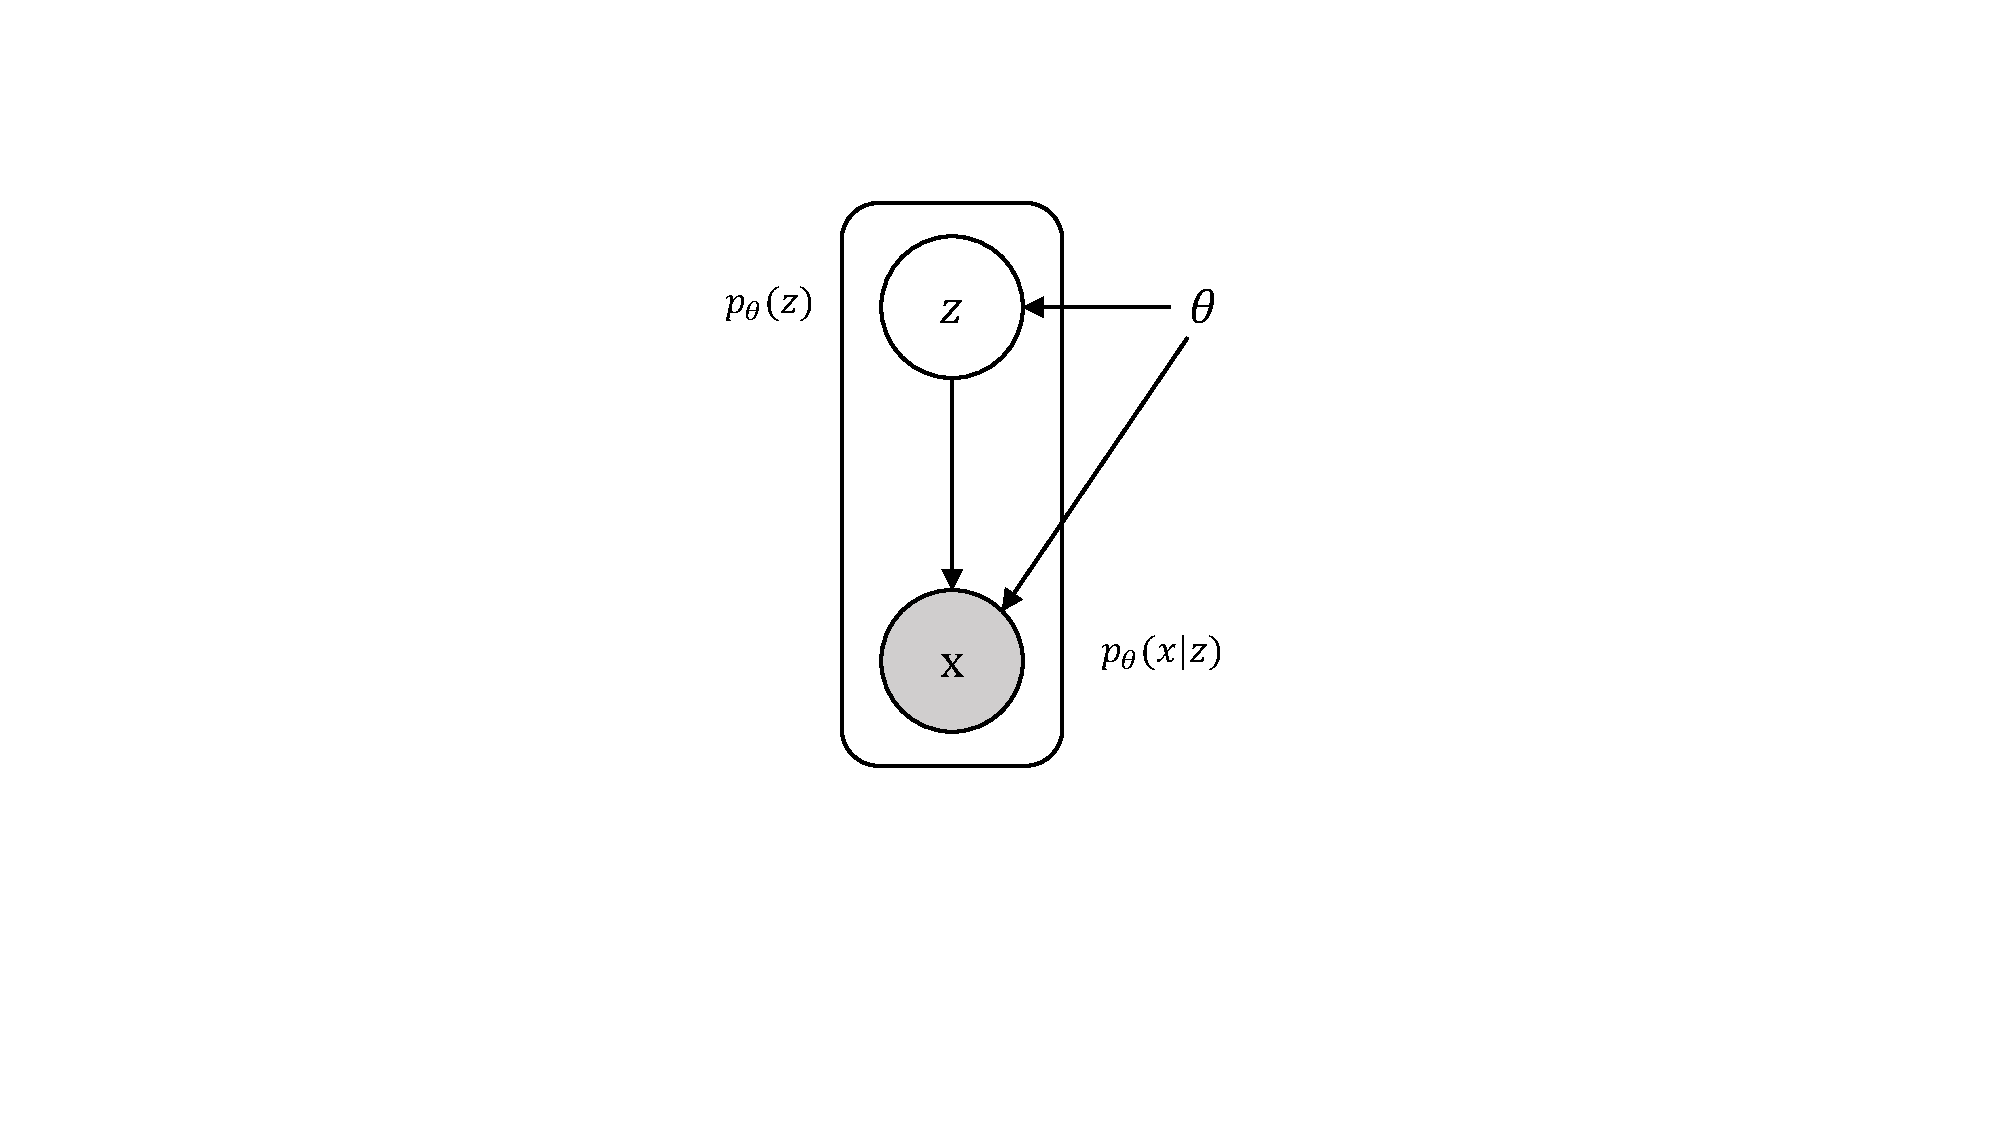
\includegraphics[width = 0.79\textwidth]{dlvm}
%\vspace{1em}
%\caption{深度隐变量模型的概率图 \label{dlvm}}
%\end{minipage}
%\centering
%\begin{minipage}[t]{0.44\textwidth}
%\centering
%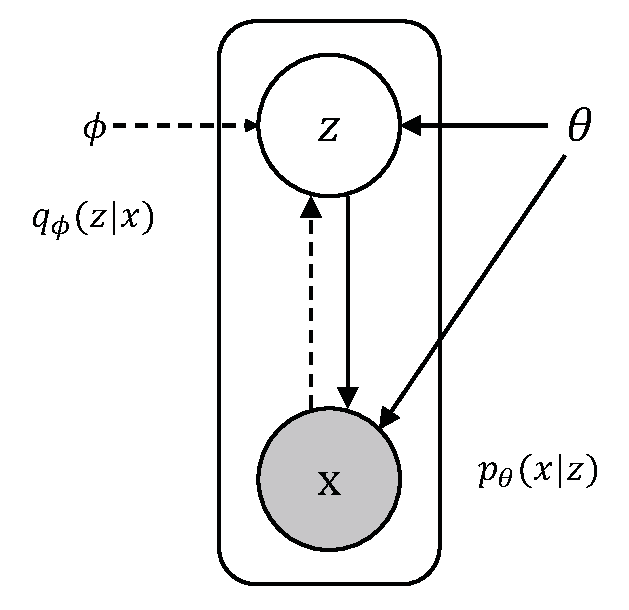
\includegraphics[width = 0.9\textwidth]{vaeg}
%\vspace{1em}
%\caption{变分自编码器的概率图 \label{vaeg}}
%\end{minipage}
%\end{figure}

\subsection{近似后验}
为了解决深度隐变量模型中无法求解后验概率分布$p_{\theta}(z|x)$的问题,Kingma\cite{kingma2013auto}等人提出了变分自编码器架构,即使用参数化的推断模型$q_{\phi}(z|x)$(编码器)来近似$p_{\theta}(z|x)$,其概率图如图\ref{vaeg}所示。我们一般使用神经网络来参数化近似后验。例如,假设后验分布满足各项同性的高斯分布,则有:
\begin{equation}
\begin{split}
	(\mu, log\sigma) & = Encoder_{\phi}(x) \\
	q_{\phi}(z|x) & = \mathcal{N}(z;\mu, diag(\sigma)) .
\end{split}
\end{equation}

\begin{figure}[htbp] 
	\centering 
	\subfigure[深度隐变量模型]{
		\begin{minipage}[htbp]{0.44\textwidth}
			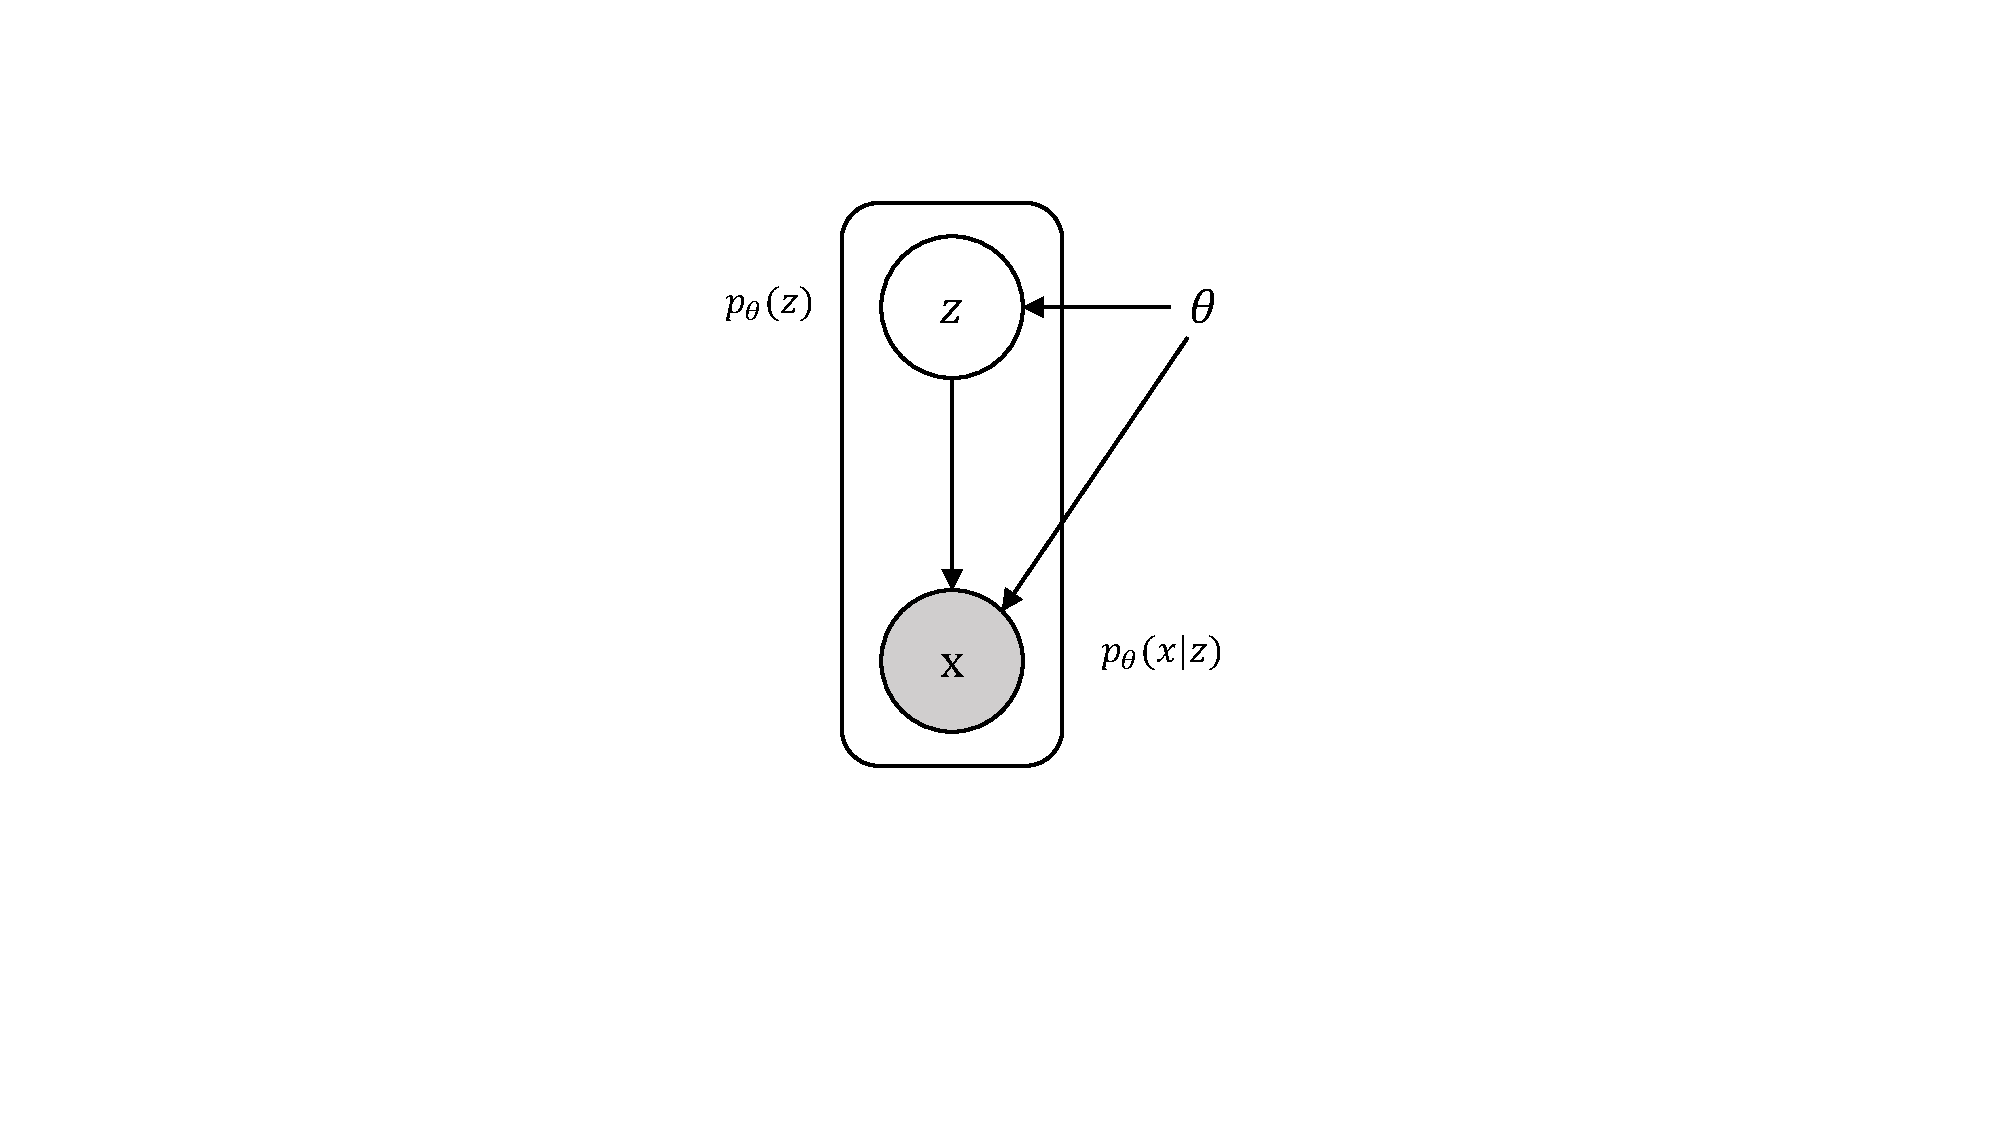
\includegraphics[width=0.79\textwidth]{dlvm} \label{dlvm}
		\vspace{0.5em}
		\end{minipage}	
	}
	\subfigure[变分自编码器]{
		\begin{minipage}[htbp]{0.44\textwidth}
			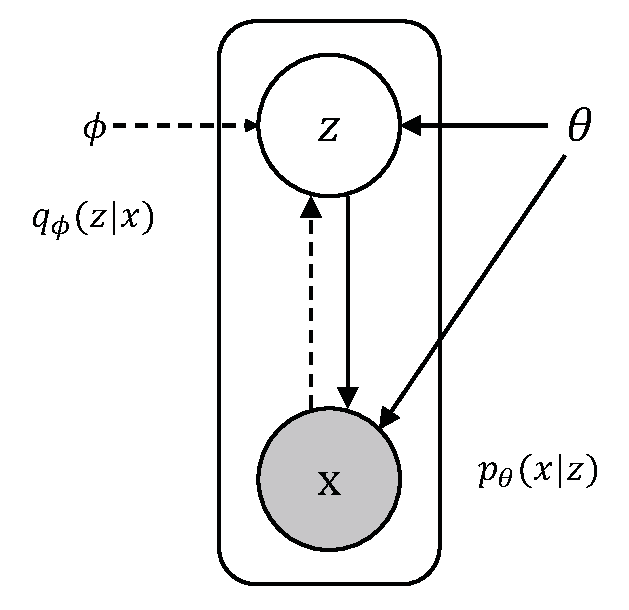
\includegraphics[width=0.9\textwidth]{vaeg} \label{vaeg}
		\vspace{0.5em}
		\end{minipage}
	}
	\caption{概率图}
\end{figure}

\subsection{变分下界}
变分自编码器的目标函数通过最大化观测变量$x$的边缘似然得到,具体推导过程如下所示:
\begin{equation}
\begin{split}
	\log{p_{\theta}(x)} & = \log{p_{\theta}(x, z)} - \log{p_{\theta}(z|x)} \\
	& = \log{\frac{p_{\theta}(x, z)}{q_{\phi}(z|x)}} + \log{\frac{q_{\phi}(z|x)}{p_{\theta}(z|x)}} \\
	& = \underbrace{\mathbb{E}_{q_{\phi}(z|x)}\bigg[\log{\frac{p_{\theta}(x, z)}{q_{\phi}(z|x)}}\bigg]}_{\mathcal{L}_{\theta, \phi}(x)} + \underbrace{\mathbb{E}_{q_{\phi}(z|x)}\bigg[\log{\frac{q_{\phi}(z|x)}{p_{\theta}(z|x)}}\bigg]}_{D_{KL}(q_{\phi}(z|x)\parallel p_{\theta}(z|x))\geq 0} \\
	& \geq \mathbb{E}_{q_{\phi}(z|x)}\bigg[\log{\frac{p_{\theta}(x, z)}{q_{\phi}(z|x)}}\bigg], \label{likehood}
\end{split}
\end{equation} 
上式第二项为$q_{\phi}(z|x)$与$p_{\theta}(z|x)$的Kullback-Leibler散度,它非负并且只有两个分布相等时等于0;上式第一项为$\log{p_{\theta}(x)}$的下界,又叫证据下界(Evidence Lower Bound,ELBO),将其展开又可得到:
\begin{equation}
	\mathcal{L}_{\theta, \phi}(x) = \log{p_{\theta}(x)} - D_{KL}(q_{\phi}(z|x)\parallel p_{\theta}(z|x)). \label{elbo}
\end{equation}

从式子\eqref{likehood}和式子\eqref{elbo}中可以发现,KL散度$D_{KL}(q_{\phi}(z|x)\parallel p_{\theta}(z|x))$决定了两种距离,第一是近似后验$q_{\phi}(z|x)$与后验$p_{\theta}(z|x)$的距离,第二是边缘似然$\log{p_{\theta}(x)}$与证据下界ELBO的距离,因此,只要保证$D_{KL}(q_{\phi}(z|x)\parallel p_{\theta}(z|x))$足够小,那么ELBO就越接近$p_{\theta}(z|x)$,也就越能代表它作为变分自编码器的目标函数。

\subsection{变分下界的梯度下降优化}
对于变分自编码器的目标函数$\mathcal{L}_{\theta, \phi}(x)$,可以采用随机梯度下降(Stochastic Gradient Descent,SGD)来更新参数$\theta$ 和 $\phi$。

参数$\theta$的梯度很容易求得:
\begin{equation}
	\begin{split}
		\nabla_{\theta}\mathcal{L}_{\theta, \phi}(x) &= \nabla_{\theta} \mathbb{E}_{q_{\phi}(z|x)}[\log{p_{\theta}(x, z)} - \log{{q_{\phi}(z|x)}}] \\
		&= \mathbb{E}_{q_{\phi}(z|x)}[\nabla_{\theta}(\log{p_{\theta}(x, z)} - \log{{q_{\phi}(z|x)}})] \\
		&\approx \nabla_{\theta}(\log{p_{\theta}(x, z)}).
	\end{split}
\end{equation}

但参数$\phi$的梯度因为ELBO的期望包含了后验分布$q_{\phi}(z|x)$,而它是关于参数$\phi$的函数 ,所以并不易算,如下所示:
\begin{equation}
	\begin{split}
		\nabla_{\phi}\mathcal{L}_{\theta, \phi}(x) &= \nabla_{\phi} \mathbb{E}_{q_{\phi}(z|x)}[\log{p_{\theta}(x, z)} - \log{{q_{\phi}(z|x)}}] \\
		&\neq \mathbb{E}_{q_{\phi}(z|x)}[\nabla_{\phi}(\log{p_{\theta}(x, z)} - \log{{q_{\phi}(z|x)}})],
	\end{split}
\end{equation}
Kingma\cite{kingma2013auto}等人巧妙地使用了重参数化技巧(Reparameterization Trick)使得ELBO可直接进行求导,主要的思想是用一个随机变量$\epsilon$与隐变量$z$建立可导的映射关系$g$,这样就可以将$z$的随机性转移到$\epsilon$上,经重参数化后的ELBO可以被重写成:
\begin{equation}
	\begin{split}
		\mathcal{L}_{\theta, \phi}(x) &= \mathbb{E}_{q_{\phi}(z|x)}[\log{p_{\theta}(x, z)} - \log{{q_{\phi}(z|x)}}] \\
		&= \mathbb{E}_{p(\epsilon)}[\log{p_{\theta}(x, z)} - \log{{q_{\phi}(z|x)}}],
	\end{split}
\end{equation}
其中$z=g(\epsilon, \phi, x)$,$\epsilon$一般服从简单的标准正太分布。

\section{本章小结}
本章介绍了基于变分自编码器进行交通缺失值填充算法设计中所需要用到的背景知识和相关理论。首先介绍了城市交通网络和缺失值填充领域中的一些重要定义,包括栅格数据和数据缺失机制;接下来介绍了神经网络中常见的卷积运算,从普通卷积到转置卷积,最后介绍了能处理时空特征的3D卷积;紧接着介绍了用于提升隐变量分布复杂性的标准化流技术;最后着重阐述了变分自编码器的相关理论,从概率图模型的角度讲述了其目标函数的由来以及对其目标函数参数的优化,本章内容的阅读有助于读者对之后章节内容的深入理解。


% Local Variables:
% TeX-master: "../thesis"
% TeX-engine: xetex
% End: